% This is samplepaper.tex, a sample chapter demonstrating the
% LLNCS macro package for Springer Computer Science proceedings;
% Version 2.20 of 2017/10/04
%
\documentclass[runningheads]{llncs}
%
\usepackage{hyperref}
\usepackage[dvipsnames]{xcolor}
\usepackage[colorinlistoftodos,prependcaption,textsize=tiny]{todonotes}
\usepackage{graphicx}
\usepackage{microtype}
\usepackage[utf8]{inputenc}
\usepackage{algorithm}
\usepackage[noend]{algpseudocode}
\usepackage{tabularx}
\usepackage{booktabs}
\usepackage{paralist}
\usepackage{subfig} 
\usepackage{etoolbox}


\hypersetup{
	pdftoolbar=true,        % show Acrobat?s toolbar?
	pdfmenubar=true,        % show Acrobat?s menu?
	pdffitwindow=false,     % window fit to page when opened
	pdfstartview={FitH},    % fits the width of the page to the window
	pdftitle={Complex Event Processing under Constrained Resources},    % title
	pdfauthor={},     % author
	pdfsubject={},   % subject of the document
	pdfcreator={},   % creator of the document
	pdfproducer={}, % producer of the document
	pdfkeywords={}, % list of keywords
	pdfnewwindow=true,      % links in new window
	colorlinks=true,       % false: boxed links; true: colored links
	linkcolor=Brown,          % color of internal links (change box color
	%with
	%linkbordercolor)
	citecolor=OliveGreen,        % color of links to bibliography
	filecolor=magenta,      % color of file links
	urlcolor=NavyBlue           % color of external links
}

\renewcommand{\labelitemi}{$\circ$}
\renewcommand{\labelitemii}{$-$}

\renewcommand*\sectionautorefname{Section}
\renewcommand*\subsectionautorefname{Section}
\renewcommand*\subsubsectionautorefname{Section}


\makeatletter
\providecommand{\subtitle}[1]{% add subtitle to \maketitle
	\apptocmd{\@title}{\par {\large #1 \par}}{}{}
}
\makeatother

% Used for displaying a sample figure. If possible, figure files should
% be included in EPS format.
%
% If you use the hyperref package, please uncomment the following line
% to display URLs in blue roman font according to Springer's eBook style:
% \renewcommand\UrlFont{\color{blue}\rmfamily}

\begin{document}
%
\title{Secure Multi-Party Computation for Inter-Organizational Process Mining}
%
%\titlerunning{Abbreviated paper title}
% If the paper title is too long for the running head, you can set
% an abbreviated paper title here
%
\author{Gamal Elkoumy\inst{1} \and
Stephan A. Fahrenkrog-Petersen\inst{2}\and
Marlon Dumas\inst{1} \and\\ Peeter Laud\inst{3} \and Alisa Pankova\inst{3} \and 
Matthias Weildich\inst{2}}
%
\authorrunning{G. Elkoumy et al.}
% First names are abbreviated in the running head.
% If there are more than two authors, 'et al.' is used.
%
\institute{University of Tartu, Tartu, Estonia \\
	\email{\{gamal.elkoumy,marlon.dumas\}@ut.ee} \and
Humboldt-Universität zu Berlin,  Berlin, Germany
\email{\{fahrenks,weidlima\}@hu-berlin.de} \and 
Cybernetica, Tartu, Estonia\\
\email{\{peeter.laud,alisa.pankova\}@cyber.ee}
}

%
\maketitle              % typeset the header of the contribution
%
\begin{abstract}
Process mining is a family of techniques for analysing business processes based 
on event logs extracted from information systems. Mainstream process mining 
tools are designed for intra-organizational settings, insofar as they assume 
that an event log is available for processing as a whole. The use of such tools 
for inter-organizational process analysis is hampered by the fact that such 
processes involve independent parties who are unwilling to, or sometimes 
legally prevented from, sharing detailed event logs with each other. In this 
setting, this paper proposes an approach for constructing and querying a common 
type of artefact used for process mining, namely the time-annotated 
directly-follows graph~(DFG), over multiple event logs belonging to different 
parties, in such a way that the parties do not share the event logs with each 
other. The proposal leverages an existing platform for 
secure multi-party computation, namely Sharemind. 
%The paper shows that a direct 
%implementation of a DFG construction algorithm in Sharemind suffers from 
%scalability issues. 
%To tackle this shortcoming, the paper proposes a 
%divide-and-conquer approach, 
%wherein the log is broken down into sub-logs that are processed in a 
%map-reduce 
%style. 
Since a direct 
implementation of DFG construction in Sharemind suffers from 
scalability issues, the paper proposes to rely on vectorization of 
event logs and to employ a divide-and-conquer scheme for parallel 
processing of sub-logs. 
The paper reports on an experimental evaluation that tests the 
scalability of the approach on real-life logs.

%processes involve independent, and sometimes mutually untrusted parties, which 
%are not willing to openly share all their business process execution data with 
%others.
%a query engine that has unfettered access to the enterprise system databases.
%tools for process mining assume that the tool has unfettered access to the entire event log. 

\keywords{Process Mining  \and Privacy \and Secure Multi-Party Computation}
\end{abstract}
%
%
%

\section{Introduction}

Analysing business processes based on event logs extracted from information 
systems through process mining techniques~\cite{Aalst16} becomes increasingly 
popular in industry. It enables organizations to optimize their processes and 
achieve their strategic goals, e.g., realizing cost-efficient process 
execution. However, 
%The rapid adoption of process mining 
%in industry is due to the tremendous potential of the technology. 
in practise, many business processes are not restricted to a single 
organization, but are executed by several collaborating organizations. 
We call such processes inter-organizational business processes.
An example of such a process is given in  
\autoref{fig:ground_handling_process}, which illustrates the ground handling of 
an aircraft, which includes at least the 
airline and the ground handler, e.g., the airport. 

\begin{figure}[t!]
	\centering
	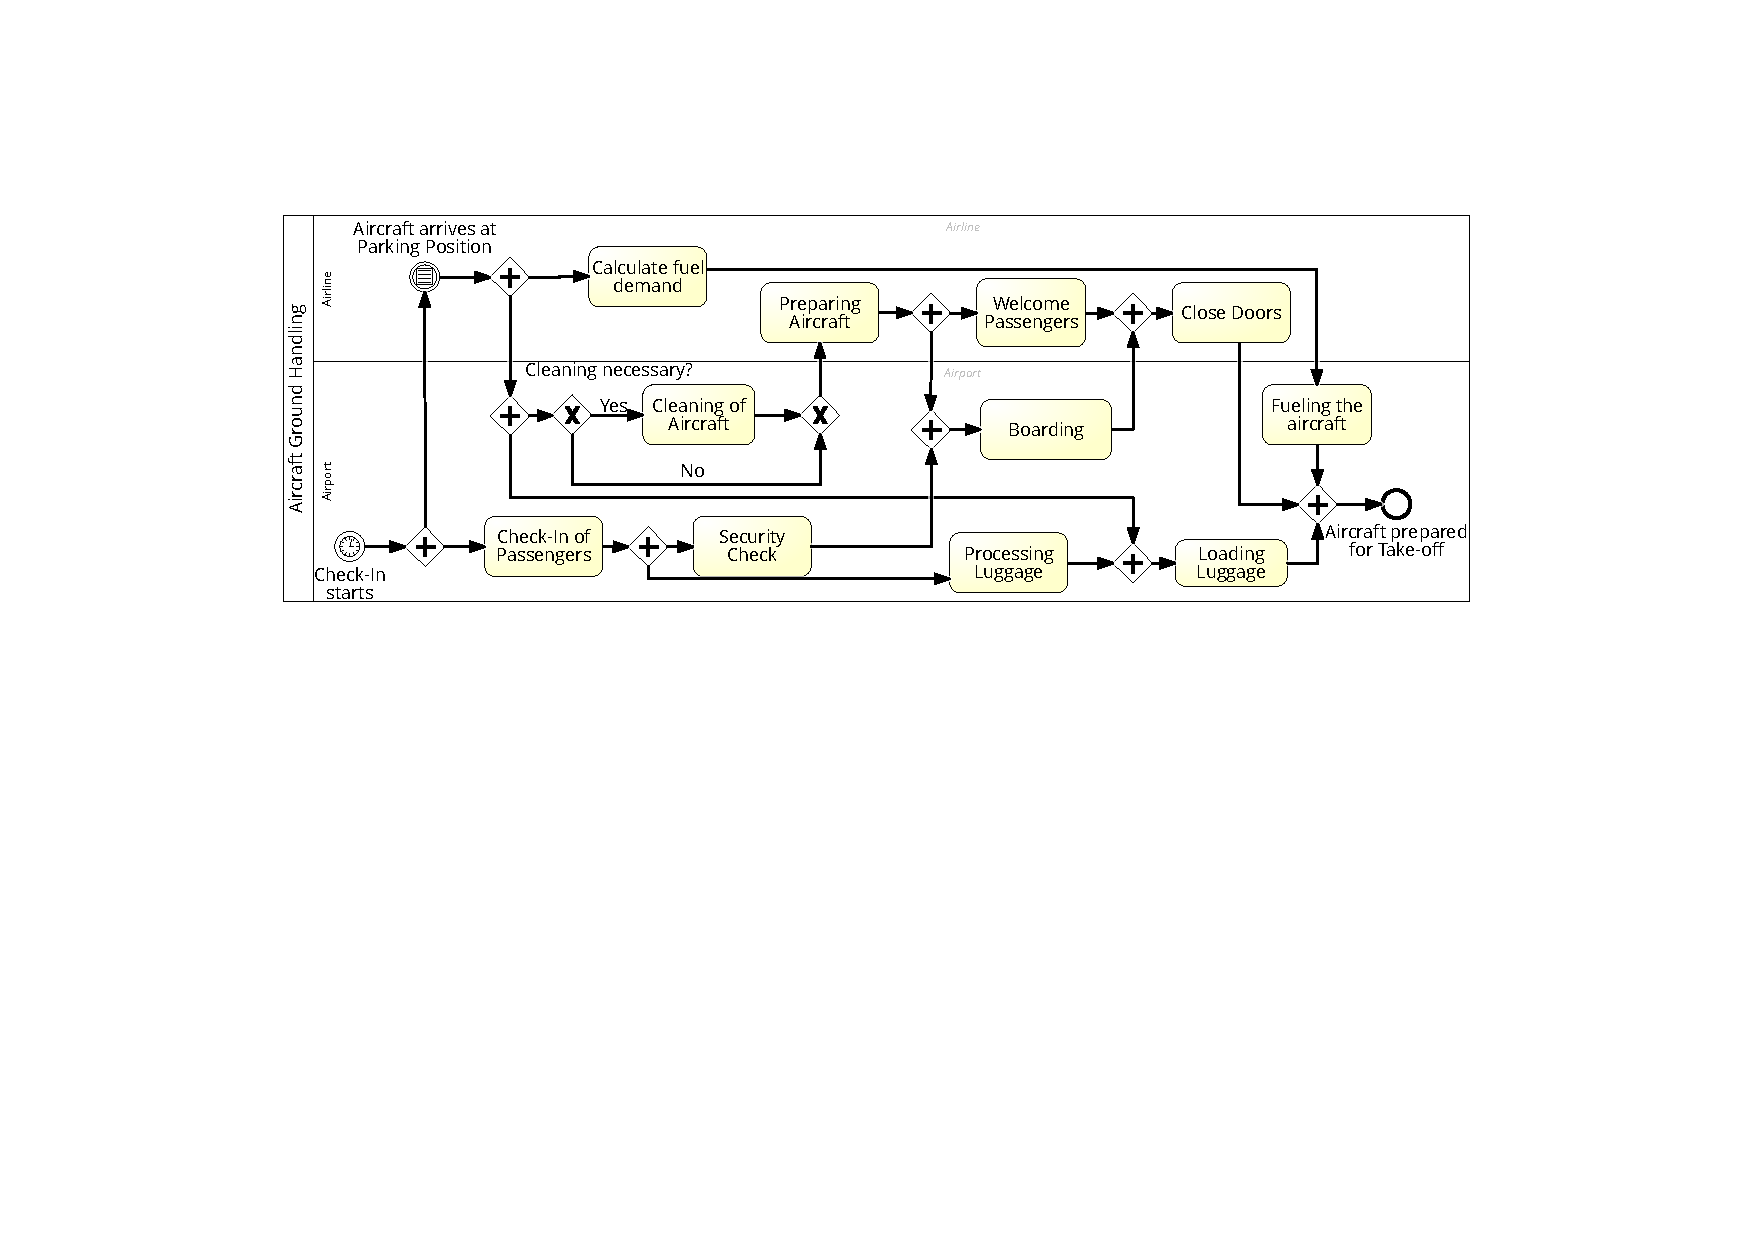
\includegraphics[width=0.98\textwidth]{figures/aircraft_ground_handling_process}
	\caption{The example of an aircraft ground handling process.}
	\label{fig:ground_handling_process}	
	\vspace{-.6em}
\end{figure}


Due to confidentiality issues and privacy regulations, such as GDPR, it is not 
possible for organizations to share their process data with each 
other~\cite{gdpr}. 
Exchanging event logs could reveal personal information of customers or expose 
business secrets. As a consequence, common techniques for process mining cannot 
be employed for inter-organizational business processes, despite the fact that 
these processes can have a large impact of the core operation of a business.
For the aforementioned scenario, for instance, it is well-known that the 
orchestration of ground handling activities is of crucial importance for both 
involved parties~\cite{schmidberger2009ground}. It determines the number of 
flights an airport can operate as well as the number of flights an airline can 
offer per aircraft. 

%Therefore, they lack this powerful tool, if the industry 
%tries to optimize these cross-organizational processes, since process mining 
%is 
%based on the analysis of so called  event logs. Datasets  that contain the 
%data 
%recorded while executing the business process. Nonetheless 
%cross-organizational 
%processes can have a high impact of the core operation of a business, such as 
%the ground handling of an aircraft is essential\cite{schmidberger2009ground} 
%for the number of flights an airport can operate. Therefore, the lack of 
%possibility to apply process mining techniques to cross-organizational 
%business 
%processes is undesirable.

%we are going to introduce a technique to enable organizations to analyse their 
%cross-organizational business processes\cite{van2011intra} without the 
%necessity to share their private data or the need of a trusted third party. 

In this paper, we focus on the question of how to enable process mining for 
inter-organizational business processes without requiring the involved parties 
to share their private event logs or trust a third party.
To this end, we propose an architecture for process mining based 
on \emph{secure multi-party computation}~(MPC)~\cite{yao1982protocols}. In essence, MPC aims 
at the realization of some computation over data from multiple parties, while
exposing only the result of the computation, but keeping the input data 
private. 
%While only enabling the input parties to gain knowledge about the public 
%outputs of the computation. 
We consider the setting of an MPC platform where the 
involved parties upload their event logs to a network of compute nodes. 
Before the upload, secret sharing algorithms locally 
split each single data value into different parts (i.e., shares) that are then 
stored at different nodes. Since each share does not provide any 
information about the original data, the uploaded event log is encrypted and 
exposed neither to the platform operator nor other involved parties. 
Nonetheless, the MPC platform enables the computation over the encrypted data 
through protocols for result sharing among the nodes. 

We realise the above architecture to answer analysis queries that are common in 
process mining. That is, we show how to construct a time-annotated 
directly-follows graph that serves as a starting point for process discovery 
algorithms~\cite{augusto2018automated} and the detection of performance bottlenecks~\cite{van2011time}. We 
implement our proposed architecture using the Sharemind 
platform~\cite{bogdanov2008sharemind}. In order to avoid scalability issues 
that would be imposed by a naive implementation, we employ vectorization of 
event logs and propose a divide-and-conquer scheme for parallel 
processing of sub-logs. We demonstrate the effectiveness of these optimisations 
in an experimental evaluation with real-world event logs. 

The remaining paper is structured as follows. \autoref{sec:background} lays out 
related work and the background for this work. \autoref{sec:approach} 
introduces our architecture for privacy-preserving inter-organizational process 
mining along with the optimizations needed for efficient implementation. An 
experimental evaluation is presented in \autoref{sec:evaluation}, before 
\autoref{sec:conclusion} concludes the paper. 


\section{Background and Related Work}
\label{sec:background}
The work we will present in this paper relates to the topics of privacy-preserving process mining, cross-organizational process mining  and secure multi-party computation. In the remainder of this section we will introduce related work out of these areas of research.
\subsection{Privacy-preserving Process Mining}
\label{sec:privacy_process_mining}
In the area of privacy-preserving process mining\cite{pika2019towards} two general approaches have been established\cite{caise/Fahrenkrog-Petersen19}: anonymizing the event data and directly performing privatized process mining techniques. For the anonymization of event logs from one organization techniques such as \emph{PRETSA}\cite{icpm/Fahrenkrog-Petersen19}, an algorithm to ensure the established privacy metrics $k$-anonymity\cite{sweeney2002k} and $t$-closeness\cite{li2007t}, exist. These metrics\cite{DBLP:journals/csur/WagnerE18}, based on data similarity, are widely adopted and offer protection against certain attacks, like the disclosure of the identity of individuals involved in the dataset.  The necessity of privacy-preserving process mining, due to novel legal development such as the GDPR, was recently discussed in \cite{mannhardt2018privacy}.
 Approaches based on cryptography\cite{burattin2015toward,simpda/RafieiWA18} have also been proposed. \\
 On the side of privatized process mining methods for prrivacy-preserving process discovery\cite{MannhardtKBWM19,tillem2016privacy,tillem2017mining} and the privacy-aware discovery of resource roles\cite{rafiei2019role} have been established. Recently the 
 Both privatized process mining and techniques for anonymizing event logs have been made available for a large audience with the tool ELPaaS\cite{elpaas2019}. The tool and all techniques mentioned above, with the exception of \cite{tillem2017mining}, a concerned with privacy-preserving process mining for one organization and have not yet adopted or evaluated for a cross-organizational setting. While is focussed on a cross-organizational setting \cite{tillem2017mining} it is only focused on  generating process models, while our aim is answering a wide range of queries about a business process.
 

 \subsection{Cross-Organizational Process Mining}
 \label{sec:cross_orgranizational}
The specific problem of privacy in cross-organizational process mining has been addressed in \cite{Liu19}. Liu et. al provide a framework for privacy-preserving cross-organizational process mining based on the assumption that a trusted third party exists and mostly focus on the discovery of process models. Our plan is to provide a solution for scenarios without a trusted third party and lays the focus on computing queries over distributed event logs in a privacy-preserving manner. Other approaches of cross-organizational process mining, that do not consider privacy aspects are presented in \cite{schulz2004facilitating,zeng2013cross}. Such as \cite{Liu19} it also aiming in the discovery of process models.
Another line for research\cite{aksu2016cross,buijs2011towards,van2010configurable} in cross-organizational process mining attends to compare the same process in different organizations.

 \subsection{Secure Multi-Party Computation}
 \label{sec:mpc}

 Secure Multi-party Computation (MPC)~\cite{GMW} is a cryptographic functionality that allows $n$ parties to cooperatively evaluate $(y_1,\ldots,y_n)=f(x_1,\ldots,x_n)$ for some function $f$, with the $i$-th party contributing the input $x_i$ and learning the output $y_i$, and no party or an allowed coalition of parties learning nothing besides their own inputs and outputs.
 
There exist a few different approaches for constructing MPC protocols. Using the inherently 2-party \emph{garbled circuits} (GC) approach~\cite{yao1982protocols,yao1986generate}, one of the parties encrypts each gate of the Boolean circuit representing $f$, and sends it to the other party, together with the keys corresponding to both parties' inputs. The second party decrypts a part of the representation of each gate, and learns the output of $f$ in the end. Garbled circuit based protocols have small round complexity, but tend to require more bandwidth than some of the next approaches.

Homomorphic encryption (HE)~\cite{elgamal1985public,paillier1999public} can be used to perform computations (mostly linear) on data without seeing it, and threshold homomorphic encryption~\cite{DBLP:conf/eurocrypt/CramerDN01} can be used to build a full MPC protocol. These primitives have been used for privately implementing the Alpha Algorithm for process discovery~\cite{tillem2016privacy,tillem2017mining}. Any computations on encrypted data are enabled by \emph{fully homomorphic encryption} (FHE) schemes~\cite{DBLP:conf/stoc/Gentry09}. While FHE-based approaches minimize the communication between parties, they are very computation-intensive.

Homomorphic secret sharing~\cite{blakley1979safeguarding,shamir1979share} is currently the most common basis for MPC protocols~\cite{CCD,GRR}. In such protocols, the arithmetic or Boolean circuit representing $f$ is evaluated gate-by-gate, constructing secret-shared outputs of gates from their secret-shared inputs. Each evaluation requires some communication between parties (except for addition gates), hence the depth of the circuit determines the round complexity of the protocol. On the other hand, there exist protocols with low communication complexity~\cite{DBLP:journals/ijisec/BogdanovNTW12,DBLP:conf/ccs/ArakiFLNO16,DBLP:conf/crypto/DamgardPSZ12}, allowing the secure computation of quite complex functions $f$, as long as the circuit implementing it has a low multiplicative depth.

The complexity of MPC protocols is heavily dependent on the number of parties jointly performing the computations. Hence the typical deployment of MPC has a relatively small number of \emph{computation parties} (typically just 2 or 3) actually running the protocols for evaluating gates, while an unbounded number of parties may contribute the inputs and/or receive the outputs of the computation~\cite{Kamm-thesis}. There exist frameworks that support such deployments of MPC, they have APIs to simplify the development of privacy-preserving applications~\cite{archer2018keys}. One of such frameworks is Sharemind~\cite{bogdanov2008sharemind}, whose main protocol set~\cite{DBLP:journals/ijisec/BogdanovNTW12} is based on secret-sharing among three computing parties. In this paper, we build on top of Sharemind and its large number of primitive protocols and subroutines~\cite{DBLP:conf/nordsec/BogdanovLT14}, but our techniques are also applicable to other secret sharing based MPC systems. Sharemind framework simplifies our work by offering the SecreC language~\cite{bogdanov2014domain} for programming privacy-preserving applications, abstracting away these details of cryptographic protocols that make sense to be abstracted away.


\section{Multi-Party Computation based Process Mining}
\label{sec:approach}
This section introduce our techniques for process mining based on 
secure multi-party computation. To this end, in \autoref{sec:model}, we first 
clarify our model for cross-organizational process mining including the 
required input data and the obtained analysis results. We then introduce our 
architecture for realizing the respective analysis using secure multi-party 
computation in \autoref{sec:core_approach}. In 
\autoref{sec:div_and_conq}, we focus on techniques for vectorization and 
parallelization to improve the efficiency of our approach.

\subsection{Model for Cross-organizational Process Mining}
\label{sec:model}

We consider a model in which an event log $L=\{t_1,\ldots,t_n\}$ is defined as 
a set of traces, each capturing the single execution of a business 
process. We define a trace $t$ as a finite sequence of events $t=\langle 
e_1,\ldots,e_m \rangle$. An event $e$ is defined as $e=(i,a,ts)$. It represents 
a single execution of an activity $a$ at time $ts$, where $i$ is 
a unique event identifier, i.e., $i = i'$ implies that $(i,a,ts) = 
(i',a',ts')$. We assume that events in a trace are ordered by their timestamp. 

However, for a cross-organizational business process, an event log that records 
the process execution from start to end is commonly not available. Rather, 
different parties record sub-logs that contain sub-traces, built of events that 
denote activity executions at the respective party. To keep the notation 
concise, we consider a setting in which two parties, $I_a$ and $I_b$, execute a 
cross-organizational process, e.g., the airport and the airline in our 
motivating example. Then, each of the two parties records an event log, denoted 
by $L_a$ and $L_b$. A trace $t=\langle 
e_1,\ldots,e_m \rangle\in L$ of the cross-organizational process is 
materialized as two sub-traces, $t_a \in L_a$ and $t_b \in L_b$, each being 
defined as the order-preserving projection of trace $t$ on the events that 
denote activity executions at the respective parties $I_a$ and $I_b$. We assume 
that each activity can only be executed by one of the parties, so that the 
projection of the log into sub-logs is defined unambiguously. 

For the above setting, we consider the scenario that the parties $I_a$ and 
$I_b$ want to answer some analysis queries $Q$ over the cross-organizational 
event log $L$, yet \emph{without} sharing their logs $L_a$ and $L_b$ with each 
other. 
More specifically, we focus on analysis queries that can be answered on a 
time-annotated directly-follows-graph (DFG) of the cross-organizational 
process. \todo{@Stephan, could you clarify that DFG would be kept secret in sharemind and we reveal only the answers for the queries?} In essence, the DFG captures the frequencies with which the executions 
of two activities have been observed to directly follow upon each other in a 
trace. Moreover, we consider temporal annotations of the directly-follows 
dependencies in terms of time between the respective activity executions. A 
time-annotated DFG thereby enables conclusions on the main paths of process 
execution, rarely executed paths, as well as the location of major delays in 
processing.

Formally, the time-annotated DFG is captured by an $|A| \times |A|$ matrix, 
where $A$ is the set of all possible activities of the process. Each cell 
contains a tuple $(c,\Delta)$. The counter $c$ represents the frequency with 
which a directly-follows dependency has been observed in $L$, i.e., for the 
cell $(a_1,a_2)$ it is the number of times that two events $e_1=(i_1,a_1,ts_1)$ 
and $e_2=(i_2,a_2,ts_2)$ follow each other directly in some trace of $L$. 
Furthermore, 
$\Delta$ is the total sum of the time that passed by between all occurrences of 
the respective events, i.e., $ts_2 - ts_1$ for the above events. 

In cross-organizational process mining, the aforementioned time-annotated DFG 
cannot be computed directly, as this would require the two parties to share and 
integrate their sub-logs. 


%To enable process mining in a cross-organizational setting we assume that the 
%queries the organizations want to execute can be answered by subset of the 
%elements of the annotated \emph{directly-follows-graph} (DFG) of the 
%cross-organizational process.
%Additionally, we consider that we have two input parties $I_a$ and $I_b$, such 
%as an airport and an airline in our motivational example. 
%These input parties 
%have access to there respective event logs $L_a$ and $L_b$, with $L_a \cap L_b 
%=\emptyset$. While the whole business process is represented by the event log 
%$L = L_a \cup L_b$. We define a log $L$ as a set of traces, 
%$L=\{t_1,...,t_n\}$. Each trace $t$ captures the single execution of a 
%business 
%process. We define a trace $t$ as a finite sequence of events $t=\langle 
%e_1,...,e_m \rangle$. Where is event $e$ is defined as $e=(i,a,ts) $ and 
%represents the single execution of an activity $a$ at time $ts$. With $i$ 
%being 
%the event identifier such as $i = i'$ implies that $(i,a,ts) = (i',a',ts')$. 
%For our cross-organizational setting we assume that a trace $t \in L$ 
%corresponds to subtraces $t_a \in L_a$ and $t_b \in L_b$, such as $t = t_a 
%\cup 
%t_b$. As an additional assumption we assume that an activity $a$ that is 
%executed by one party, e.g.,$I_a$, can not be executed by the other party, 
%e.g. 
%$I_b$.
%
%We assume that the input parties $I_a$ and $I_b$ want to calculate some 
%queries 
%$Q$ over the cross-organizational event log $L$ without sharing their 
%respective logs $L_a$ and $L_b$ with each other. However, to answer the 
%queries 
%in $Q$ they must generate the DFG over their combined event log $L$. The 
%annotated DFG is a matrix based on $ A \times A$, where $A$ is the universe of 
%all possible activities in $L$. Each cell of the DFG matrix contains a tuple 
%$(c,\Delta)$. The counter $c$ represents the times a 
%directly-follows-relations 
%appeared, e.g. an event $e_2$ of activity $a_2$ was executed after an event 
%$e_1$ of activity $a_1$ appeared in trace $t_1$, and the total sum of time 
%$\Delta$ that passed by between all occurrences of that 
%directly-follow-relations, so for our trace $t_1$ the time passed would be 
%$\Delta_1 = ts_2 - ts_1$ with $ ts_1 \in e_1,  ts_2 \in e_2 $.

\subsection{MPC Architecture for Process Mining}
\label{sec:core_approach}

In order to enable inter-organizational process mining based on a 
time-annotated DFG \emph{without} requiring parties to sharing their event logs 
with each other, we propose an architecture for secure multi-party computation 
(MPC). As outlined in \autoref{fig:overview}, we rely on a platform for MPC 
that takes the event logs of the participating parties, i.e., $L_a$ and $L_b$, 
as encrypted input. In the MPC platform, the respective data is then prepared 
in several steps in order to answer analysis queries over the time-annotated 
DFG. 

%Since we believe we sharing the complete DFG would reveal to much confidential 
%information in most scenarios, we would only release a subset of the cells of 
%the DFG based on some queries $Q$. 

\begin{figure}[!htb]
	\centering
	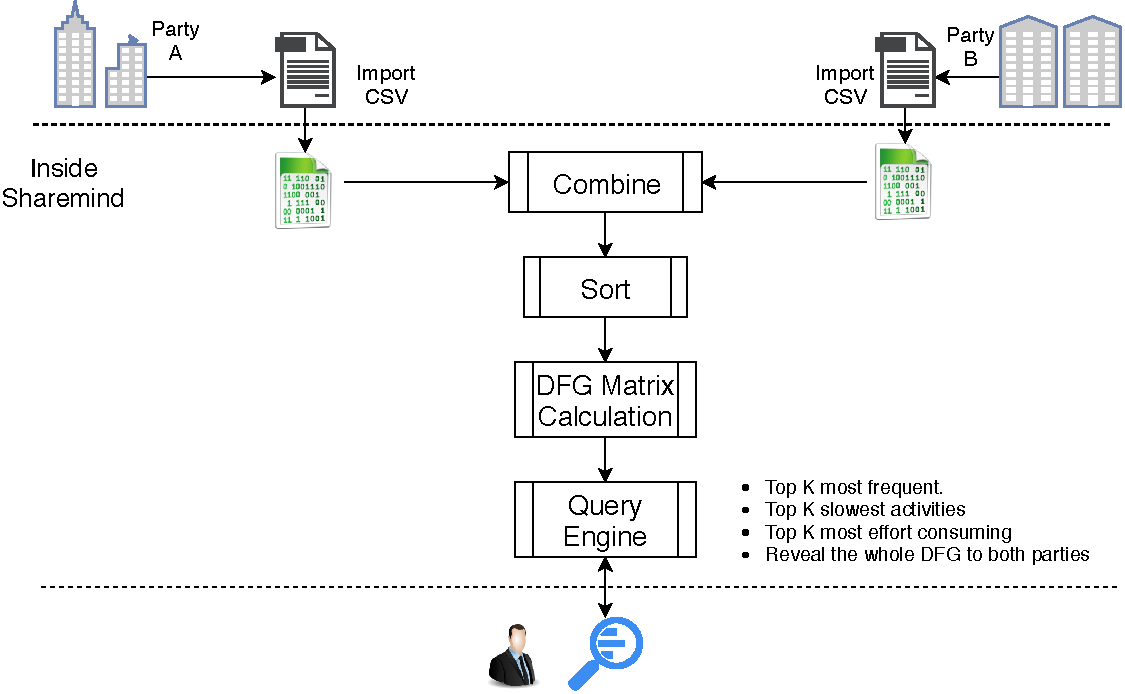
\includegraphics[width=.95\columnwidth]{figures/mpc_algorithm}
	\caption{Number of variants retained for $k$-anonymity.}
	\label{fig:overview}
\end{figure}

\noindent
We summarize the functionality realized in the MPC platform as 
follows:
\begin{compactitem}
\item[\emph{Combination}] While the input parties upload their respective event logs $L_a$ and $L_b$ to the MPC platform, these get encrypted and distributed to the computing parties. So it is ensured, that nobody can access the secret data. After the logs upload we append one of the logs to the other so that the unsorted log $L$ is created.
\item[\emph{Sorting}] To ensure an efficient calculation of the annotated DFG $G$ we sort the merged log $L$, such that all event $e \in t$ of a trace $t \in L$ are group together and ordered by their respective execution time $ts$. For this purpose we rely on the network sorting algorithm\cite{bogdanov2014practical}, that ensures efficient sorting without revealing secret information.
\item[\emph{Matrix calculation}] After sorting $L$ we can construct the DFG $G$ inside the MPC platform, while keeping the DFG $G$ secret and not revealing any information.
\item[\emph{Query answering}] A query $Q$ requests a subset $S$ of the annotated DFG $G$. The MPC platform generates $S$ based on the query $Q$, e.g., the top-5 most common activities, and only reveals this subset $S$ to the output parties. By publishing only the subsets $S$ to pre-defined output parties we limit the information an output party can learn about the process. 
\end{compactitem}

%It consists of several major steps, starting with merging the secret 
%logs $L_a$ and $L_b$ by appending them to each other and then sorting them, 
%such that all event $e \in t$ of a trace $t \in L$ are group together and 
%ordered by their respective execution time $ts$. To ensure an efficient 
%execution of such sorting we rely on the network sorting 
%algorithm\cite{bogdanov2014practical}. Following the sorting we construct the 
%DFG based on the algorithm~\ref{alg:merge}.

%After construction the combined DFG $G$ we can apply the queries $Q$ and retrieve the respective subsets $S$ of $G$. Each subset $s \in S$ represents the answer to one query $q \in Q$. By publishing only the subsets $S$ to pre-defined output parties we limit the information an output party can learn about the process. 

%\begin{algorithm}[!htb]
%	\caption{Calculating the combined, annotated DFG($L$)}
%	\label{alg:merge}
%	\begin{flushleft}
%		\textbf{INPUT:} The sorted combined event log $L$\\
%		\textbf{OUTPUT:} DFG $G$, Waiting time matrix $W$
%		\vspace{-.4em}
%	\end{flushleft}
%	\begin{algorithmic}[1]
%		\State Initialize $G$,$W$
%		\ForAll{$t \in \mathit{L}$} \label{line:all_cases}
%			\State currentEvent $\gets$ startEvent
%			\Repeat
%				\State $G_a$ = currentEvent * nextEvent($t$).reshape()
%				\State $W$ = $G_a$ *  (nextEvent($t$).timestamp - currentEvent.timestamp)
%			\Until nextEvent($t$) $ = \emptyset$ 
%		\EndFor
%		\State \Return $G$, $W$
%	\end{algorithmic}
%\end{algorithm}

%Algorithm~\ref{alg:merge} shows the respective algorithm. Our approach keeps both event logs separated and only calculates the combined DFG. Alternatively, it would be possible to merge both logs $L_a$ and $L_a$ into one log $L$ and then calculate the DFG over $L$. However, this would require sorting the merged  log $L$ based on the time an event happened, to enable calculating the DFG. But sorting has the complexity of $\mathcal{O}(n \log n)$ and our algorithm has the complexity of $\mathcal{O}(n)$, with $n$ being the number of events in $L = L_a \cup L_b$. Therefore, Algorithm~\ref{alg:merge} ensures faster performance compared to a  simple merge of $L_a$ and $L_b$.


\subsection{Scalability Considerations}
\label{sec:div_and_conq}

Cross-organizational process mining using the above general architecture might 
suffer from scalability issues. The reason being the use of multi-party 
computation to realise the functionality to combine and sort the event logs and 
to calculate the annotated DFG, which is inherently distributed and applied to 
homomorphic encrypted data. Hence, even 
for functions that have a generally low run-time complexity ($\mathcal{O}(n)$ 
for the combination, $\mathcal{O}(n\log(n))$ for the sorting, 
$\mathcal{O}(n^2)$ for 
the calculation of the annotated DFG), there is a non-negligible overhead 
induced by MPC. For instance, a naive realisation of the Quicksort algorithm to 
sort the events of the combined log would require $\mathcal{O}(n\log(n))$ 
rounds of communication between the distributed nodes and 
$\mathcal{O}(n\log(n))$ value comparisons per round~\cite{Hamada12}. Against 
this background, we consider two angles to improve the efficiency of 
the analysis, namely vectorization and parallelization. 

\paragraph{Vectorization.} Contemporary MPC platforms provide efficient 
implementations of basic functions to process distributed, encrypted data. 
For instance, Sharemind supports bitwise secret sharing that represents a data 
value as a bitwise combination of vectors that are distributed among the nodes. 
Based thereon, the platform offers efficient implementations of vector-based 
functions, such as those for matrix 
multiplication~\cite{kerik2016optimizing,laud2017privacy}. For instance, the 
multiplication of two bit vectors can be realized in one round that requires 
$\mathcal{O}(6k)$ interactions between nodes, where $k$ is the number of bits 
required to encode the value. 

To leverage the efficient implementation of such basic functions, we employ 
vectorization and represent events as a bit vector over the set $A$ of all 
possible activities of the process. To mask the actual number of possible 
activities, the set over which the vector is defined may include padding, i.e., 
some additional placeholders. Following this representation, an event 
corresponds to a binary vector in which at most one bit is set to one. Then, 
counting the number of directly-follows dependencies in the computation of the 
annotated DFG can be traced back to vector multiplication. 


\todo{Matthias, rework the following}
\paragraph{Parallelization.}
An additional approach to improve the runtime performance common for 
secure-multi party computation is the usage of parallelization. To ensure 
efficient parallelization it is important to divide the data from the input 
parties such that all data chunks can be used independent from each other. In 
our scenario this can be done by bundling chunks of cases and distributing them 
to several machine.  For each chunk a DFG can be generated. The different DFGs 
can then be united to one DFG that represents the entire business process. 

However, such an approach comes with the question of determining the size of the chunks. We consider that a chunk has size $m$ representing the number of cases that are at least part of that chunk. In a multi-party computation setting the result of the processing of each chunk would not be protected. Therefore, proceeding only a small number of cases in one chunk might reveal a lot of information about the cases inside the chunk and is critical from a privacy perspective. On the other hand comes a small chunk size $m$ with the advantage of higher performance, since it would be possible to distribute the work over more machines. This leads to an important trade-off between runtime performance and privacy considerations. 

To enable an efficient splitting of  the event log into chunks, it in necessary that all traces have the same length. If this condition is true, the sorted event log can just be split up at certain points, e.g. exactly in the middle if the aim is to generate two chunks and the number of traces is odd. Otherwise a split into chunks would require scanning the whole event log for the right point to split it, something that would come the computational cost of $\mathcal{O}(n)$, with $n$ being the events in the log. Therefore, we apply a padding to the traces in the log, so that all traces have the same length, the length of the longest trace. Such a padding can be done by each input party, if they pad their part of the trace to the length of the max length of their respective longest sub trace. Since such a preprocessing comes with lower costs, than performing additional operations in a MPC setting. Nonetheless, we need to ensure that the padding has no influence on the generated DFG. Therefore, we propose padding with a bit vector, representing the activity, containing only zeros. Thanks to our vectorization approach such as padding has no influence on the resulting DFG.
\section{Evaluation}
\label{sec:evaluation}
In this section we will provide an  evaluation for our introduced approaches based on the following research questions:
 \begin{description}
 	\item[Q1:] How do different event logs characteristics influence the performance of the secure multi-party computation?
 %	\item How does the number of chunks influence the performance of the secure multi-party computation?
 \item[Q2:] Does the proposed approach scale up with increasing the number of parallel chunks and what would be the effect of scalability on both the execution time and communication overhead between the computing parties?
\end{description}


\subsection{Datasets}
\label{sec:data}
To evaluate our approaches we run the experiment using the following real-world event logs:
\begin{description}
	\item[BPIC 2017] This event log captures the loan application process from a dutch financial institute. This event logs contains traces with a medium length, but is the largest investigated log in terms of number of events.
	\item[Traffic Fines] This event logs captures a process to handle the collection of fines from traffic law violations from a local police from Italy. It consists of rather short traces with a small number of different activities.
	%\item[Hospital Log] This event log captures treatments in a dutch hospital. The event log contains of long traces with an average of over 100 events in one trace.
		\item[Credit Requirement] This event log captures credit requirement process information in a dutch bank. The event log contains of short traces with only 8 unique events.
\end{description}
All of the introduced event logs capture a process from a single organization and not a cross-organizational business process. We decided to do so, because the existing public synthetic event logs\cite{borkowski2017event} for cross-organizational business processes consist only of a marginal number of events. Therefore, we have chosen event logs that contain a large number of cases and vary in the length of the traces, see table~\ref{tab:event_logs}. For the BPIC 2017, the data took about 5 hours till time out, we decide to selected 1000 traces randomly from the event log so we the log file could converge in a reasonable file.

To simulate  a cross-organizational setting we use Round Robin approach to assign each activity of each event log  to one party, assuming the business process is executed in a two party setting. We distribute the activities equally between both parties, so that each party executed half of the activity types for each log.

\begin{table}[!ht]
	
	\begin{tabularx}{\textwidth}{ X X X X X X}\\
		\toprule
		Event Log &No. of events &No. of cases & Avg. No. of events in case &Max No. of events in case & Min No. of events in case \\
		\midrule
		BPIC 2017 &		1,202,267 &	 31,509 & 38.16& 180 & 10\\
		Traffic Fines &	 561,470 & 	150,370 & 3.73& 20 & 2\\
		Hospital Log &	 150,291 &	 1,143 & 131.488 & 1814 & 1\\
		\bottomrule
	\end{tabularx}
	\caption{Event Logs for Evaluation}
	\label{tab:event_logs}
\end{table}

\subsection{Experimental Setup}
\label{sec:exp_setup}
To answer the above questions, we benchmark the performance of the proposed approach. We consider latency, throughput and the communication overhead as performance measures. 

\textbf{Latency.} We define latency as the amount of time needed to transform the 2 parties' event log securely into a DFG matrix. We report both the total execution time and the execution time of the chunk based sort. That would help to study how would help to study how the implementation of the proposed approach would be in a map/reduce like scheme. In subsection~\ref{sec:results}, the experiments show that changing the number of parallel chunks affects the chunk based sort only but the rest of the pipeline has a fixed execution time for the same dataset.

\textbf{Throughput.} We define throughput as the number of events that the system can process in a given amount of time. In our experiment, we report the number of events per minute as a measure of throughput.

\textbf{Communication Overhead.} In multi-party computation, the computing parties are communicating together so they can compute the final results securely. We define the communication overhead as the amount of data sent and received between the computing parties during the execution overhead. We report the values for each server. The communication overhead metric gives insights for how the system  would react in case the computing parties are remotely installed.

In the above performance measures, we perform the experiments until we have the DFG matrix, because it is the most sophisticated and time consuming portion of the pipeline, as it requires communicating both parties to build the matrix. Furthermore, once we have the DFG in secret shares, we can calculate the required queries in short time.

We provide the source code of our implementation on \emph{Github}\footnote{\url{https://github.com/Elkoumy/SecureMPCBPM}}. To implement our approaches we used the SecreC programming language from Cybernetica. Our implementation is run on the multi-party computation platform Sharemind\footnote{\url{https://sharemind-sdk.github.io}}.

To evaluate the performance of an approach we report the average maximum values for latency and the average value for both throughput the communication overhead. To calculate the mean execution time we run each experimental setting over 5 times and calculate the maximum execution time of the three servers. We used \emph{Nethogs}\footnote{\url{https://github.com/raboof/nethogs}} to measure the communication overhead and we report the average value per server.


\textbf{Hardware.} We run our experiments in a setting with three symmetrical servers as computation parties. These physical servers are connected through a local network. All of them use the same Sharemind setup. Each server has AMD Processor 6276 and 192 GB RAM and all the servers are connected using 1 gigabit Ethernet switch.


\subsection{Results}
\label{sec:results}


\begin{figure}[!htb]
	\centering
	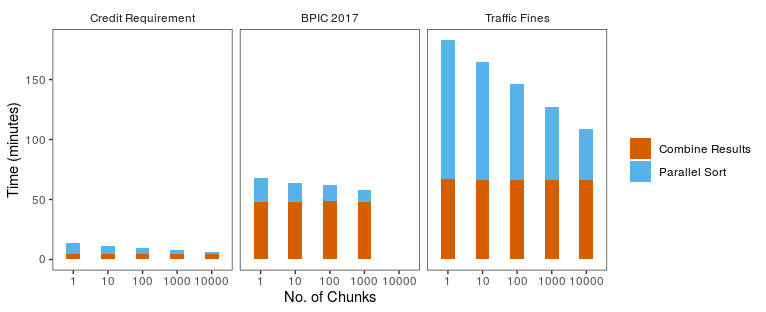
\includegraphics[width=.95\columnwidth]{figures/latency.png}
	\caption{Latency Benchmark: Execution Time vs no. of Chunks.}
	\label{fig:latency}
\end{figure}

\textbf{Latency Benchmark.} In fig~\ref{fig:latency}, we show the execution time to calculate the DFG matrix securely with different number of parallel chunks. We plot a bar for each chunk size. We split each bar to present the execution time of parallel sort in blue and the rest of the execution time in orange. From fig~\ref{fig:latency}, we can see that the execution time decreases with increasing the number of parallel chunks due to the execution of sort in parallel for each chunk separately. Because the sort complexity is $O(n log n)$, and after dividing data into chunks, the sorting complexity per chunk is $O((n/c) \: log  \: (n/c))$ where c is the number of parallel chunks. The execution time when using a single chunk, the sort is slower as c equals 1 and by increasing the number of chunks the factor $n/c$ decreases which reduces the execution time.  Furthermore, from fig~\ref{fig:latency}, we can observe that the execution time of the parallel sort, the blue part of the bars, changes with changing the number of parallel chunks and the combine results is almost fixed for each dataset. 

An interesting observation is that, both Credit Requirement and Traffic Fines datasets as the same number of events, and different number of unique events. The number of unique events increases the number of bits used to represent the event in the binary representation for the outer product step. Increasing the number of unique events per log makes the result matrix bigger which adds computation overhead. The same thing could be observed with the BPIC 2017 dataset as it has larger number of unique events.


\begin{figure}[!htb]
	\centering
	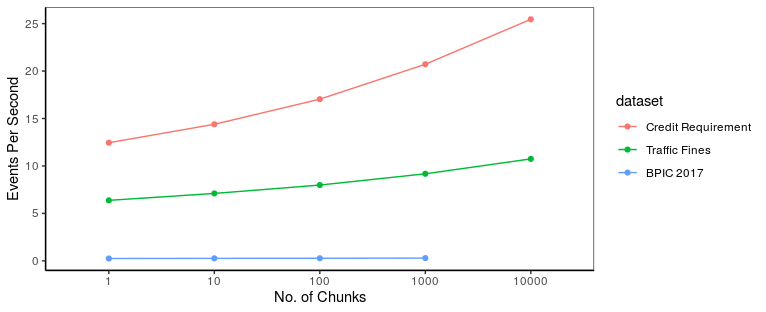
\includegraphics[width=.95\columnwidth]{figures/throughput.png}
	\caption{Throughput Benchmark: Events per Second vs no. of Chunks.}
	\label{fig:throughput}
\end{figure}

\textbf{Throughput Benchmark.} In fig~\ref{fig:throughput}, we report the number of events per second for different number of chunks. We can observe that, for datasets with smaller average number of events per trace, as in the Traffic Fines log, the throughput increase largely with increasing the number of chunks. However, increasing the average number of events per trace, as in both Credit Requirement log and BPIC 2017 log, makes the throughput grows slower. The reason for that is with the larger average of events per trace, the size of the data grows rapidly because of padding. We choose padding to avoid revealing the number of events per each trace.
%\begin{figure}[!htb]
%	\centering
%\subfloat[Data Sent]{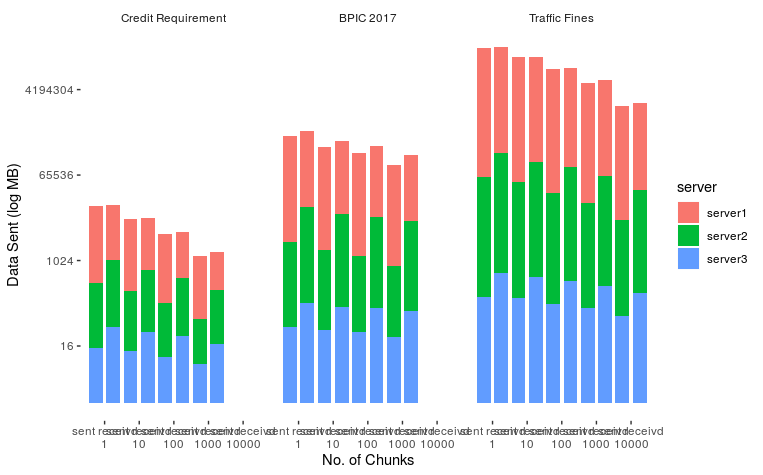
\includegraphics[width=0.5\textwidth, keepaspectratio]{figures/communication.png}\label{fig:comm_sent}}
%\subfloat[Data Received]{\includegraphics[width=0.5\textwidth, keepaspectratio]{figures/communication_received.png}\label{fig:comm_reveived}}

%\caption[]{Data Sent and Received for different servers vs the number of Chunks.}
%\label{fig:comm}
%\end{figure}

\begin{figure}[!htb]
	\centering
	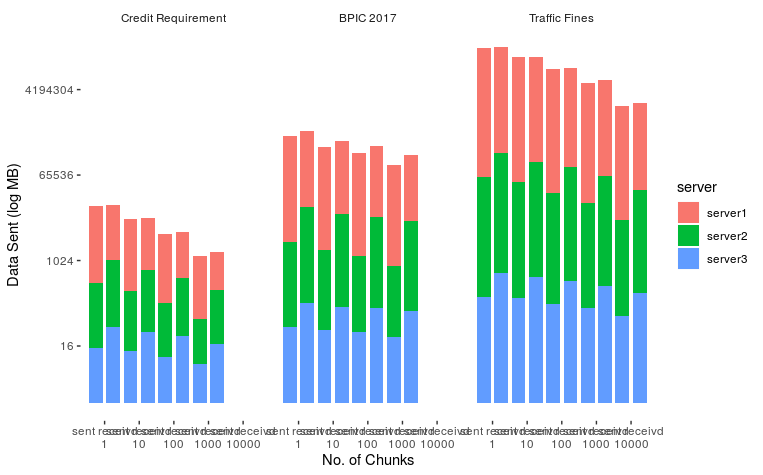
\includegraphics[width=.95\columnwidth]{figures/communication.png}
	\caption{Communication Benchmark: Data Sent and Received vs no. of Chunks.}
	\label{fig:comm}
\end{figure}

\textbf{Communication Overhead Benchmark.} In fig~\ref{fig:comm} , we present the amount of data sent and received at each server. We can observe that the communication overhead decreases with increasing the number of chunks. There are differences between the values reported for the different servers, because our implementation inside Sharemind uses asymmetry of comparison protocols.

Also, we can observe from fig~\ref{fig:comm} that the communication overhead increases with increasing the number of unique events per event log. That happens as the outer product for larger matrix size costs more communications. 



\section{Conclusion}
\label{sec:conclusion}
This paper introduces a framework for inter-organizational process mining based on secure multi-party computation. Our approach enables organizations to perform process mining on shared business processes with revealing only the number of traces per log, the number of unique events and the maximum number of events per a trace. To ensure a scalable execution of the secure multi-party computation we introduce techniques based on vectorization and divide-and-conquer. Our evaluation on real world event logs shows that these technique improve the performance of the secure multi-party computation and scale up under different characteristics of event logs.

Several directions for future research arise such as combining our approach with privacy guarantees like differential privacy to comply with stronger privacy requirements. Additionally, it could be explored how an adversarial input can be prohibited from gaining knowledge by manipulating the secure multi-party computation with false input data.

 \bibliographystyle{splncs04}
 \bibliography{bib_mpc_process_discovery}

\end{document}
